\subsection{Proof of Concept for Future Research}
\subsubsection{Comparative Analysis Tool}
As we proceeded with the interviews, the library selection factors and process were maturing early in the research phase (after around 8th interview). We have frequently heard from the interviewees about the variation of priorities of different library selection factors. Depending on particular situation of the target application, under diverse organizational culture and team dynamics, developers often change the priorities. We decided to apply our analyzed findings to see if that would help developers.

Following our findings, we started discussing with the interview practitioners regarding an applicable tool that can be used in the industry. We experimented with a dynamic weight mechanism for each decision making factor. Developers can customize such factors based on their situation and by calculating a weighted average of all necessary factors of alternative libraries, developers can finally come to a more structured method of their library comparison. 

After the 8th interview, we designed a mock user interface (UI) for comparative analysis with weight of factors and demonstrated the interface to the subsequent interviewees. A sample comparison between two Java libraries Jackson and Gson for JSON data processing is presented from the mock UI in the Figure \ref{fig:ui-library-comparison}.
\begin{figure*}
    \centering
    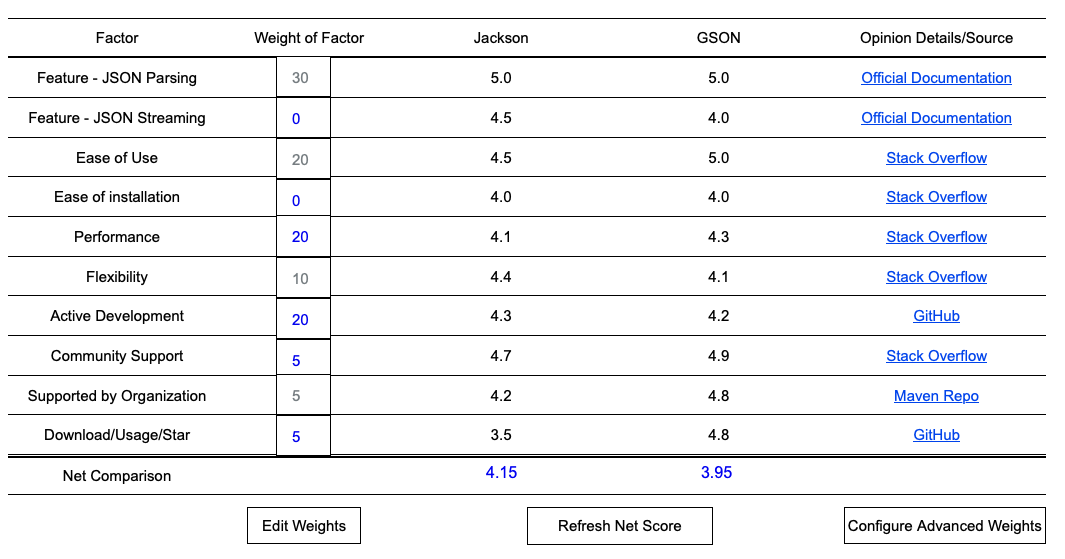
\includegraphics[scale=0.4]{images/mock-ui-library-comparison.png}
    \caption{A sample comparative analysis of two libraries by mining large scale data from source code repository and question-answer sites.}
    \label{fig:ui-library-comparison}
\end{figure*}

The first column in the comparison chart contains few decision making functional and technical factors. The second column Weight of Factors takes input weights from the developers for their particular situation. The scores under two libraries' columns (Jackson and Gson) contains an aggregated score from the data analysis on respective factors. For example, to measure the score of ease of use, we would be mining developers' sentiment in Stack Overflow regarding the specific libraries and come up with the score out of five based on the positive or negative comments shared there. Some scores can be populated using quantitative data collection such as extracting Star (favorite) or measuring recent development activity from GitHub. We would also share the reference of the actual sources from which we are measuring this score in the last column Opinion Details/Source. The final outcome of the analysis is the net comparison of weighted average score of two libraries shown in the bottom summary line. We also envisions advanced configuration of the weight of factors can be designed later on.

All the interviewees highly appreciated such structured approach of a highly subjective decision that they need to take on a regular basis. We assume that a future research work can implement the large scale online review mining and summarize the performance of libraries following this proposed comparative analysis to provide a helpful tool to the developers.


\subsubsection{Relative Priorities of Library Selection Factors}
During our interviews while we discussed about library selection factors, we often asked developers whether they treat all the factors equally important. All participants unanimously expressed that all the factors have different priorities to them in general. That was also one motivation to provide weight of the factors in the comparison tool described in previous section. Though we explained in detail that guiding principles influence the library selection factors to great deal, we realized that a generic priority of library selection criteria would be helpful for developers' common understanding and for implementation of any comparative analysis tool.

% Table generated by Excel2LaTeX from sheet 'Priority of factors'
\begin{table}[htbp]
  \centering
  \caption{Relative priorities of library selection factors. The higher score reflects higher priority practitioners put on when selecting a third party library. The priority score is normalized out of 10. Our recommended cut-off factors are marked with asterisk (*).}
    \begin{tabular}{llr}
    \toprule
    \textbf{Factor} & \textbf{Category} & \multicolumn{1}{l}{\textbf{Priority}} \\
    \midrule
    Performance & Software &                 8.2  \\
    Stability & Software &                 7.8  \\
    Licence* & Commercial &                 7.5  \\
    Documentation & Commercial &                 7.3  \\
    Security* & Software &                 6.9  \\
    Compatibility* & Software &                 6.4  \\
    Active Development & Maintenance &                 6.2  \\
    Popularity & External &                 6.0  \\
    Supported by Own Organization & Maintenance &                 5.9  \\
    Ease of Use & Software &                 5.5  \\
    Capability of Library* & Software &                 5.5  \\
    Dependency & Commercial &                 5.4  \\
    Flexibility & Software &                 5.4  \\
    Open Source Software & Commercial &                 5.2  \\
    Community Support & Maintenance &                 5.2  \\
    Cost  & Commercial &                 5.1  \\
    Used by Reputed Companies & Maintenance &                 4.9  \\
    Availability of Demo & Commercial &                 4.8  \\
    Large Community & Maintenance &                 4.5  \\
    Supported by Reputed Organization & Maintenance &                 4.4  \\
    Customer Support & Maintenance &                 4.4  \\
    Familiarity & External &                 4.3  \\
    Size of Library & Software &                 4.2  \\
    Search Engine Ranking & External &                 4.1  \\
    Ease of Installation & Software &                 3.6  \\
    Interesting Interface & Software &                 2.7  \\
    Detailed Benchmark & External &                 2.6  \\
    Roadmap & Commercial &                 2.4  \\
    \bottomrule
    \end{tabular}%
  \label{tab:factor-priority}%
\end{table}%

In this regard, during the member checking survey (described in quality evaluation section), we also asked our interview participants how they compare among all the 28 library selection factors. For each factor, we let them choose a score in a sliding scale of 20. We used "Statement randomization" feature of Qualtrics software to randomize the list of the selection factors so that respondents do not get biased by the survey list \cite{website:replication-package}. 

\td{9} out of \td{11} respondents of the survey provided their scoring of relative priorities of library selection criteria. The Table \ref{tab:factor-priority} shows the average priority of selection factors normalized in the scale of 10. Participants chose Performance, Stability, License, Documentation, and Security as their top priority factors. Though we observed that the guiding principles can significantly influence the priority of these factors, we recommend Security and License to be 'cut-off' factors for any team so that they do not compromise with non-supported license and security vulnerabilities. We observed that two other factors 'Capability of Library' and 'Compatibility' are also cut-off factors in the sense that if a library is not compatible with target environment and does not perform the intended task, there is no point in using such a library. We marked these four factors with asterisk to denote them as cut-off factors in the Table \ref{tab:factor-priority}. We believe, any future research could enhance this generic priority of factors to a more customized priority score followed by the guiding principles to respect the conditions of particular organization and development team.
